% !TEX program = tectonic
% FICHE 10 v6 — « chercheur » : 6 pages, chiffres remplis depuis le notebook exécuté
\documentclass[10pt,a4paper,landscape]{article}
\usepackage[margin=0.8cm]{geometry}
\usepackage[T1]{fontenc}
\usepackage[utf8]{inputenc}
\usepackage{lmodern}
\usepackage[french]{babel}
\usepackage{amsmath,amssymb}
\usepackage{booktabs,tabularx}
\usepackage{xcolor}
\usepackage{graphicx}
\usepackage{tikz}
\usetikzlibrary{positioning,arrows.meta}
\definecolor{bleu}{RGB}{20,77,144}
\definecolor{vert}{RGB}{20,110,60}
\definecolor{vertc}{RGB}{90,168,120}
\definecolor{orange}{RGB}{196,123,0}
\definecolor{rouge}{RGB}{160,30,30}
\definecolor{grisf}{RGB}{100,100,100}
\newcommand{\chb}{{\color{bleu}\rule{2.1mm}{2.1mm}}}
\newcommand{\chv}{{\color{vert}\rule{2.1mm}{2.1mm}}}
\newcommand{\cho}{{\color{orange}\rule{2.1mm}{2.1mm}}}
\pagestyle{empty}
\setlength{\parindent}{0pt}
\begin{document}

% ══════════ PAGE 1 — QU'EST-CE QU'ON TESTE ? ══════════
\begin{center}
{\LARGE\bfseries Copier les portefeuilles du Congrès avec des données complètes}\\[0.6mm]
{\small l'ancienne stratégie ne lisait que les PTR et partait de portefeuilles vides --- on répare les deux trous de données et on mesure chaque réparation isolément\\
House 2014-2026 $\cdot$ notebook \texttt{Portefeuilles\_House\_Complet} (autonome, 61 cellules exécutées, chaque chiffre sort d'une cellule) $\cdot$ 11 années civiles vs SPY, seuil $t_{10} \approx 1{,}81$}
\end{center}
\vspace{1mm}

\begin{center}
\begin{tikzpicture}[x=1cm, y=1cm,
  b/.style 2 args={rectangle, rounded corners=3pt, draw=#1, fill=#1!8, thick,
                   text width=#2, align=center, inner sep=6pt, font=\small},
  fl/.style={-{Stealth[length=3mm]}, very thick, draw=grisf}]

% bandeau KPI
\node[b={grisf}{25.8cm}] at (13.4, 15.4)
  {\textbf{128\,960} trades ({\color{bleu}107\,976 PTR} $+$ {\color{orange}20\,984 O/A/T}) \quad$\cdot$\quad
   \textbf{437} membres qui tradent \quad$\cdot$\quad {\color{vert}\textbf{160}} portefeuilles d'entrée injectés \quad$\cdot$\quad
   \textbf{11} années d'évaluation};

% ── gauche : la frise d'un trade ──
\node[font=\small\bfseries, anchor=west] at (0.6, 13.6) {La vie d'une information (et ce que l'ancienne stratégie en voyait)};
\draw[->, thick, grisf] (0.8, 11.8) -- (12.6, 11.8);
\fill[grisf] (1.6, 11.8) circle (0.09);
\node[font=\scriptsize, align=center] at (1.6, 11.3) {transaction\\ $\tau$};
\fill[bleu] (4.1, 11.8) circle (0.11);
\node[font=\scriptsize\bfseries, text=bleu, align=center] at (4.1, 12.5) {PTR\\ $\sim$27 j};
\fill[orange] (10.6, 11.8) circle (0.11);
\node[font=\scriptsize\bfseries, text=orange, align=center] at (10.6, 12.5) {rapport annuel O/A/T\\ $\sim$374 j};
\fill[vert] (2.6, 11.8) circle (0.11);
\node[font=\scriptsize\bfseries, text=vert, align=center] at (2.85, 10.9) {photo Schedule A au dépôt $f_0$ :\\ tout le patrimoine, une fois};
\node[b={grisf}{11.6cm}, anchor=north west] at (0.6, 10.0)
  {{\scriptsize l'ancienne stratégie $=$ la flèche {\color{bleu}\textbf{bleue}} seule, et chaque portefeuille reconstruit
   \textbf{à partir de zéro} --- symptôme : \textbf{937 M\$} de ventes déclarées qu'elle ne peut pas exécuter (le stock n'existe pas dans ses données)}};

% ── droite : la matrice 2×2 ──
\node[font=\small\bfseries, anchor=west] at (14.2, 13.6) {Le design : 4 runs, même stratégie, seules les données changent};
\node[b={grisf}{4.6cm}] (cA) at (17.6, 11.4) {\textbf{A} --- témoin\\ {\scriptsize\chb\ PTR seuls, départ zéro}\\ \textbf{226} membres};
\node[b={orange}{4.6cm}] (cC) at (23.4, 11.4) {\textbf{C}\\ {\scriptsize\chb\cho\ $+$ trades O/A/T}\\ \textbf{380} membres};
\node[b={vert}{4.6cm}] (cB) at (17.6, 8.9) {\textbf{B}\\ {\scriptsize\chb\chv\ $+$ photos d'entrée}\\ \textbf{257} membres};
\node[b={bleu}{4.6cm}] (cD) at (23.4, 8.9) {\textbf{D} --- adaptée\\ {\scriptsize\chb\chv\cho\ les deux}\\ \textbf{400} membres};
\node[font=\scriptsize, text=orange, anchor=south] at (23.4, 12.6) {$+$ O/A/T $\rightarrow$};
\node[font=\scriptsize, text=vert, rotate=90, anchor=south] at (15.9, 8.9) {$+$ photo $\rightarrow$};

% ── contrastes ──
\node[b={grisf}{25.8cm}] at (13.4, 6.4)
  {\textbf{l'identification} :\quad B $-$ A $=$ \textbf{\color{vert}effet photo}\qquad C $-$ A $=$ \textbf{\color{orange}effet O/A/T}\qquad
   D $-$ B $-$ C $+$ A $=$ \textbf{interaction}\\[0.4mm]
   {\scriptsize même stratégie dans les 4 cases : classement Sharpe (éligible $n_j \ge 126$ et Sharpe $> 0{,}4$) $\cdot$ $K^*$ walk-forward $\cdot$ poids $1/K$ $\cdot$ tenue 1 an --- rien d'autre ne bouge}};

% ── verdict ──
\node[b={rouge}{25.8cm}] at (13.4, 4.4)
  {\textbf{le résultat en deux phrases} : aucun run ne bat le SPY ($\max t = 0{,}85$) et les trades O/A/T pèsent négativement ($-2{,}2\,\%$/an apparié).
   MAIS la vérification par les rapports annuels (p.\,5) montre que la reconstruction adaptée est presque \textbf{10$\times$ plus complète} : rappel des positions déclarées 6\,\% $\to$ 57\,\%, à précision égale};

\node[font=\scriptsize, text=grisf] at (13.4, 3.0)
  {p.\,2 les livres de comptes $\cdot$ p.\,3 les membres : qui a quoi $\cdot$ p.\,4 la mécanique d'un membre $\cdot$
   \textbf{p.\,5 la vérification par les O} $\cdot$ p.\,6 le verdict stratégie $\cdot$ p.\,7 l'autopsie du $+6{,}6\,\%$ $\cdot$ p.\,8 conclusion};

\end{tikzpicture}
\end{center}

\newpage
% ══════════ PAGE 2 — LES LIVRES DE COMPTES ══════════
\begin{center}
{\Large\bfseries 2 $\cdot$ D'où sortent les chiffres ? Les livres de comptes, marche par marche}\\[0.5mm]
{\scriptsize chaque marche est une cellule du notebook avec assert d'identité (total $-$ marches $=$ retenu) --- rien n'est écarté sans raison affichée}
\end{center}

\begin{center}
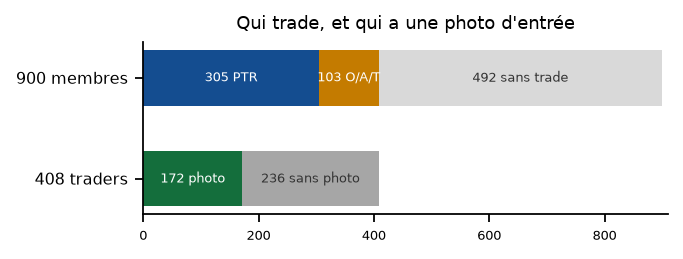
\includegraphics[width=0.66\textwidth]{figures/fig_10_partition.png}
\end{center}

\noindent\begin{minipage}[t]{0.32\textwidth}\vspace{0pt}
{\color{orange}\rule{3mm}{3mm}}\ \textbf{\color{orange}Trades O/A/T : 26\,115 $\to$ 20\,984}
\begin{center}\scriptsize
\begin{tabular}{@{}lr@{}}
\toprule
lignes table 16 (sans écho PTR) & 26\,115 \\
$-$ exchanges (sens E) & $-221$ \\
$-$ dates hors 2013-2026 & $-14$ \\
$-$ sans montant & $-0$ \\
$-$ ticker corrompu (garde-fou) & $-48$ \\
$-$ aucune série de prix$^{\dagger}$ & $-4\,367$ \\
$-$ collision exacte avec nos PTR$^{\ddagger}$ & $-481$ \\
\midrule
\textbf{= retenus (provenance oat)} & \textbf{20\,984} \\
\bottomrule
\end{tabular}
\end{center}
{\scriptsize $^{\dagger}$ après tentative de téléchargement — EIF puis les fonds monétaires (SPAXX, FZDXX, FDRXX\ldots). $^{\ddagger}$ 490 appariements : 9 lignes matchent 2 lots PTR du même jour.\\
$\approx$ 16\,\% du flux total.}
\end{minipage}\hfill
\begin{minipage}[t]{0.32\textwidth}\vspace{0pt}
{\color{bleu}\rule{3mm}{3mm}}\ \textbf{\color{bleu}Membres : 900 $\to$ 437 qui tradent}
\begin{center}\scriptsize
\begin{tabular}{@{}lr@{}}
\toprule
membres dans la table 16 brute & 370 \\
$-$ aucune ligne O/A/T exploitable & $-33$ \\
\quad {\color{grisf}dont repêchés par leurs PTR} & {\color{grisf}15} \\
\quad {\color{grisf}dont vraiment sortis} & {\color{grisf}18} \\
\midrule
= membres O/A/T exploitables & 337 \\
\quad dont : ont aussi des PTR & 205 \\
\quad dont : \textbf{O/A/T seulement} & \textbf{132} \\
$\cup$ membres PTR (non-régression : identique) & 305 \\
\midrule
\textbf{= population qui trade} & \textbf{437} \\
\bottomrule
\end{tabular}
\end{center}
{\scriptsize assert : $900 = 305 + 132 + 463$ (ne tradent pas) $\cdot$ partition photo : $166 + 271 = 437$.}
\end{minipage}\hfill
\begin{minipage}[t]{0.32\textwidth}\vspace{0pt}
{\color{vert}\rule{3mm}{3mm}}\ \textbf{\color{vert}Photos : 284 $\to$ 160 injectées}
\begin{center}\scriptsize
\begin{tabular}{@{}lr@{}}
\toprule
photos déposées (1 par membre, 252 H $+$ 32 C) & 284 \\
$-$ aucune ligne tickérisée et valorisée & $-36$ \\
\midrule
= photos exploitables & 248 \\
$-$ aucun prix au 1\ier{} jour coté $\geq$ dépôt & $-20$ \\
\midrule
= membres initialisables ($h_0$ construit) & 228 \\
\quad dont : tradent $\to$ \textbf{injectés} & \textbf{160} \\
\quad dont : aucun trade (rien à simuler) & 68 \\
\bottomrule
\end{tabular}
\end{center}
{\scriptsize 75,3\,\% de la valeur des photos convertie en parts $\cdot$ par membre : médiane 387\,505 \$, max 78,3 M\$ $\cdot$ B injecte le sous-ensemble PTR (117), D les 160.}
\end{minipage}

\vspace{2mm}
\noindent\begin{minipage}[t]{0.51\textwidth}\vspace{0pt}
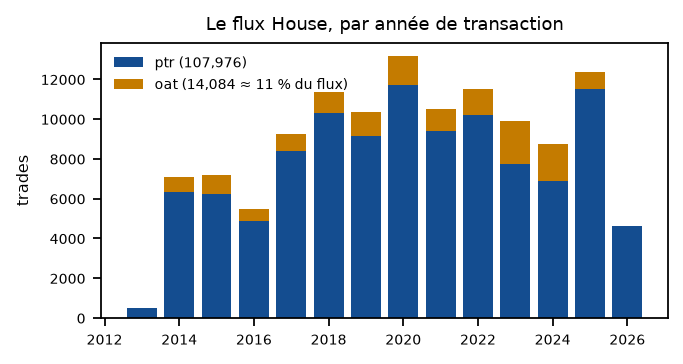
\includegraphics[width=\linewidth]{figures/fig_10_flux.png}
\end{minipage}\hfill
\begin{minipage}[t]{0.46\textwidth}\vspace{0pt}
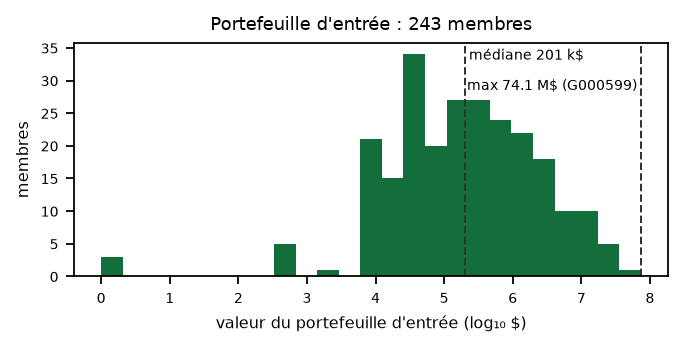
\includegraphics[width=\linewidth]{figures/fig_10_h0_couverture.png}
\end{minipage}

\vspace{0.5mm}
{\scriptsize\color{grisf} v7 : l'univers de prix couvre désormais AUSSI les tickers O/A/T (avant, $\sim$6\,000 trades étaient écartés \og sans prix \fg{} alors que le prix existait ou était téléchargeable — bug réparé, PTR inchangés au trade près) $\cdot$ preuves : sha256 $\equiv$ manifeste, map tickers 0 conflit, fourchettes écart 0.}

\newpage
% ══════════ PAGE 3bis — LES MEMBRES : QUI A QUOI ══════════
\begin{center}
{\Large\bfseries 3 $\cdot$ Les membres : qui a quoi comme information ?}\\[0.5mm]
{\scriptsize la matrice d'information (900 membres $\times$ 6 sources, cellule P1) résumée en typologie --- et les deux natures d'information : signal rapide (PTR) vs enregistrement annuel (O/A/T)}
\end{center}

\noindent\begin{minipage}[t]{0.40\textwidth}\vspace{0pt}
\textbf{Typologie (partition exhaustive des 900)}
\begin{center}\small
\begin{tabular}{@{}lr@{}}
\toprule
équipés \textbf{complets} (photo $+$ trades $+$ O $+$ T) & \textbf{49} \\
photo $+$ trades $+$ O (pas encore de T) & 113 \\
trades $+$ photo OU O (partiels) & 257 \\
trades seulement & 18 \\
aucun trade exploitable & 463 \\
\midrule
total registre & 900 \\
\bottomrule
\end{tabular}
\end{center}
\begin{itemize}
\item[--] \textbf{459 membres} ont $\geq 1$ photo annuelle O exploitable (2\,173 documents) --- c'est l'assiette de la vérification p.\,5 ;
\item[--] les délais recalculés : \textbf{PTR 27 j} (q90 49) vs \textbf{O/A/T 373 j} (q90 540) --- le PTR est un signal, l'annuel un enregistrement ;
\item[--] la matrice complète (par membre : photo ? n PTR ? n O/A/T ? années O ? T ?) est affichée dans le notebook.
\end{itemize}
\end{minipage}\hfill
\begin{minipage}[t]{0.57\textwidth}\vspace{0pt}
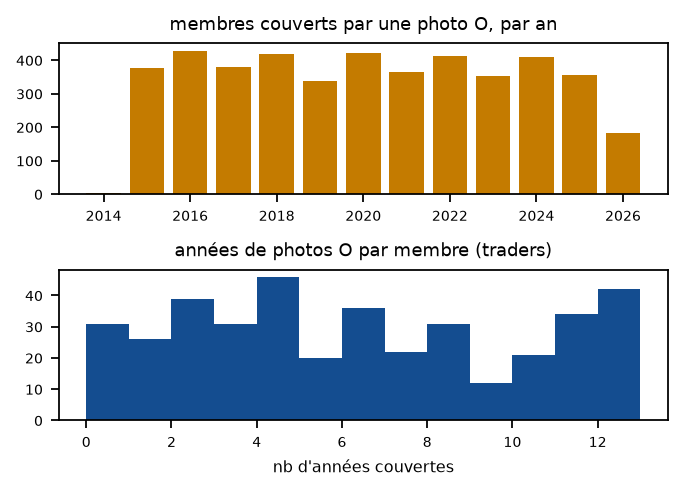
\includegraphics[width=\linewidth]{figures/fig_10_couverture_O.png}\\[1mm]
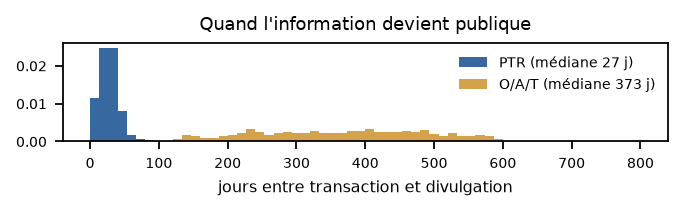
\includegraphics[width=\linewidth]{figures/fig_10_delais.png}
\end{minipage}

\newpage
% ══════════ PAGE 3 — QU'EST-CE QUE ÇA CHANGE POUR UN MEMBRE ? ══════════
\begin{center}
{\Large\bfseries 4 $\cdot$ Qu'est-ce que ça change pour un membre --- et donc pour le classement ?}\\[0.5mm]
{\scriptsize en 10 secondes : la photo change le point de départ et rend les ventes exécutables ; le Sharpe mesuré change ; le top-K change à toutes les coupes}
\end{center}

\noindent\begin{minipage}[t]{0.44\textwidth}\vspace{0pt}
\textbf{Les maths, en trois lignes.} Pour un membre $m$, ticker $i$ (parts $h$) :
$$h_0(m,i) = \tilde v_i / P_i(\tau(f_0)) \quad \text{au jour du \textbf{dépôt}}$$
$$\text{achat : } h \mathrel{+}= \tilde v / P(\tau(t)) \qquad \text{vente : } h \mathrel{-}= \min(q, h)$$
$$r_m(t) = \frac{\sum_i h_i(t{-}1) P_i(t)}{\sum_i h_i(t{-}1) P_i(t{-}1)} - 1 \quad \text{(parts de la \textbf{veille})}$$
{\scriptsize $\tilde v$ = milieu de fourchette $\cdot$ un apport n'est jamais une performance ($r = 0$ exactement au jour d'injection, testé) $\cdot$ rendements bornés $\pm50\,\%$/j.}

\vspace{2mm}
\textbf{Le mécanisme, en chiffres :}
\begin{itemize}
\item[--] le témoin A élimine \textbf{79} membres, dont \textbf{77 vendeurs purs} (que des ventes : en partant de zéro, jamais de portefeuille) --- la photo en \textbf{ressuscite 31} dans B ;
\item[--] à la coupe 2021 : \textbf{152} éligibles dans A, \textbf{241} dans D ($+$95 entrants, $-$6 sortants) --- le scatter ci-contre montre qui bouge et pourquoi ;
\item[--] conséquence : la sélection du top-$K$ diffère entre A et D à \textbf{11 coupes sur 11}.
\end{itemize}

\vspace{2mm}
{\scriptsize\color{grisf} validations du moteur : recalcul naïf en double boucle $=$ 869 rendements identiques $\cdot$ B $\equiv$ A pour les membres sans photo $\cdot$ bloc 2018 de la stratégie recalculé à la main $\equiv$ moteur.}
\end{minipage}\hfill
\begin{minipage}[t]{0.53\textwidth}\vspace{0pt}
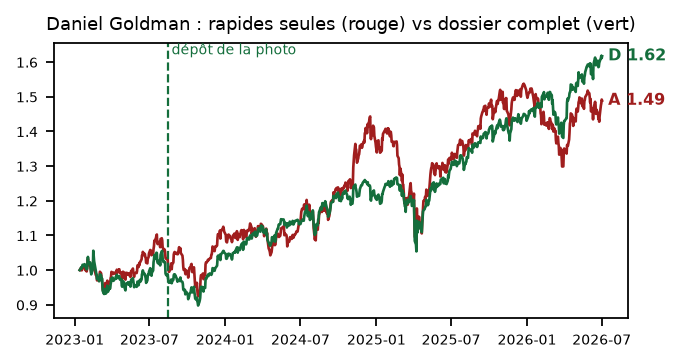
\includegraphics[width=\linewidth]{figures/fig_10_filrouge.png}\\[1mm]
\begin{center}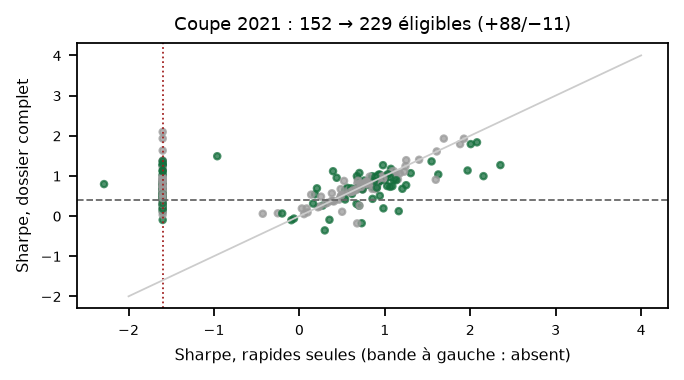
\includegraphics[width=0.78\linewidth]{figures/fig_10_sharpe_shift.png}\end{center}
\end{minipage}

\newpage
% ══════════ PAGE 5 — LA VÉRIFICATION PAR LES O ══════════
\begin{center}
{\Large\bfseries 5 $\cdot$ La vérification : les rapports annuels jugent la reconstruction}\\[0.5mm]
{\scriptsize en 10 secondes : le témoin ne retrouve que 6\,\% des positions que les élus déclarent chaque année --- la reconstruction adaptée en retrouve 57\,\%, à précision égale}
\end{center}

\noindent\begin{minipage}[t]{0.42\textwidth}\vspace{0pt}
\textbf{La méthode.} Chaque photo O déclare le patrimoine au 31/12 ; à la date de \textbf{dépôt} de l'O
(1\ier{} jour coté $\geq$ f), on confronte la reconstruction h(t) à la déclaration :
\begin{itemize}
\item[--] \textbf{(a) positions} : précision = part du reconstruit qui est déclaré ; rappel = part du déclaré qu'on a reconstruit ;
\item[--] \textbf{(b) valeurs} : sur les positions communes, $h \cdot P \in [\underline v, \bar v]$ ?
\end{itemize}
Assiette : \textbf{2\,173 photos O} $\cdot$ 459 membres $\cdot$ 3\,242 confrontations (A et D).

\vspace{2mm}
\textbf{Le verdict}
\begin{center}\small
\begin{tabular}{@{}lccc@{}}
\toprule
 & A témoin & D adaptée & \\
\midrule
rappel médian & 6\,\% & \textbf{57\,\%} & $\nearrow\nearrow$ \\
précision médiane & 60\,\% & 59\,\% & $\approx$ \\
valeurs en fourchette & 53\,\% & 52\,\% & $\approx$ \\
\bottomrule
\end{tabular}
\end{center}
\begin{itemize}
\item[--] le \textbf{T} en réconciliation finale : 122 photos de sortie, rappel 63\,\%, précision 60\,\% ;
\item[--] validation : une photo recomptée à la main $\equiv$ la table (assert) ;
\item[--] limites : clés ticker seulement $\cdot$ fourchettes larges $\cdot$ photo au 31/12 confrontée au jour du dépôt (bruit symétrique A/D) $\cdot$ amendements non re-fusionnés.
\end{itemize}
\textbf{La lecture} : les corrections (photo d'entrée $+$ trades O/A/T) rendent le portefeuille reconstruit
presque \textbf{10$\times$ plus complet} sans dégrader la justesse --- c'est la preuve, indépendante de toute
performance boursière, que l'exploitation des filing types améliore la donnée.
\end{minipage}\hfill
\begin{minipage}[t]{0.55\textwidth}\vspace{0pt}
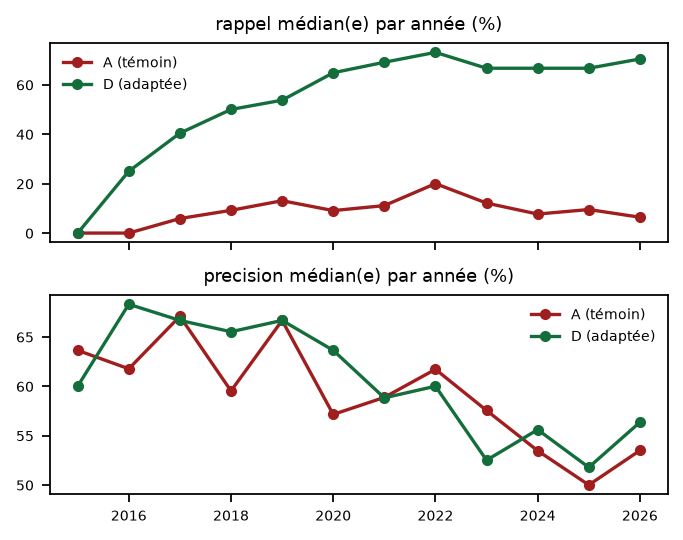
\includegraphics[width=\linewidth]{figures/fig_10_verif_O.png}\\[0.5mm]
{\scriptsize rappel (gauche) et précision (droite) médians par année : l'écart de rappel est massif et stable sur toute la période ---
le témoin, qui part de zéro et ne voit que les PTR, passe à côté de l'essentiel du patrimoine déclaré.}
\end{minipage}

\newpage
% ══════════ PAGE 4 — LE VERDICT CHANGE-T-IL ? ══════════
\begin{center}
{\Large\bfseries 6 $\cdot$ Le verdict stratégie change-t-il ?}\\[0.5mm]
{\scriptsize en 10 secondes : trois courbes qui finissent ensemble, aucun $t$ au-dessus du seuil --- non. Et le test apparié, plus puissant, dit non aussi.}
\end{center}

\noindent\begin{minipage}[t]{0.46\textwidth}\vspace{0pt}
\textbf{Le tableau central} {\scriptsize(poids $1/K$ ; 11 années ; seuil $t_{10} \approx 1{,}81$)}
\begin{center}\small
\begin{tabular}{@{}lrrlrrr@{}}
\toprule
run & excès/an & $t$ & gagn. & $\beta$ & $\alpha$/an & $t_{\text{ap}}$ \\
\midrule
\chb\ A témoin & $+0{,}9\,\%$ & $0{,}37$ & 4/11 & $0{,}99$ & $+0{,}6$ & $0{,}28$ \\
\chb\chv\ \textbf{B} & $\mathbf{+6{,}6\,\%}$ & $\mathbf{0{,}85}$ & 5/11 & $0{,}98$ & $+5{,}2$ & $\mathbf{1{,}55}$ \\
\chb\cho\ C & $-1{,}3\,\%$ & $-0{,}77$ & 3/11 & $0{,}83$ & $+1{,}0$ & $0{,}65$ \\
\chb\chv\cho\ \textbf{D} adaptée & $-1{,}6\,\%$ & $-0{,}61$ & 6/11 & $0{,}85$ & $+0{,}6$ & $0{,}37$ \\
\bottomrule
\end{tabular}
\end{center}
{\scriptsize note : pondération inverse-vol jouée partout --- elle perd sur les 4 runs ; $1/K$ reste le défaut.}

\vspace{2mm}
\textbf{Les effets, testés en différences appariées} {\scriptsize($d_Y = x_Y(\text{run}) - x_Y(A)$, mêmes années, même SPY --- test plus puissant que les $t$ marginaux)}
\begin{center}\small
\begin{tabular}{@{}lrr@{}}
\toprule
effet & moyenne (\%/an) & $t$ apparié \\
\midrule
photo (B$-$A) & $+5{,}7$ & $0{,}74$ \\
O/A/T (C$-$A) & $-2{,}2$ & $-0{,}74$ \\
interaction (D$-$B$-$C$+$A) & $-6{,}0$ & $-0{,}89$ \\
\bottomrule
\end{tabular}
\end{center}
\textbf{Message : $\max t = 0{,}85$ --- indiscernable de zéro, même apparié.}\\[0.5mm]
{\scriptsize l'essentiel du $+6{,}6\,\%$ de B vient d'\textbf{une seule année} : 2020, excès $+82{,}5\,\%$ (barres ci-contre) --- d'où le $t$ faible malgré la moyenne.}
\end{minipage}\hfill
\begin{minipage}[t]{0.51\textwidth}\vspace{0pt}
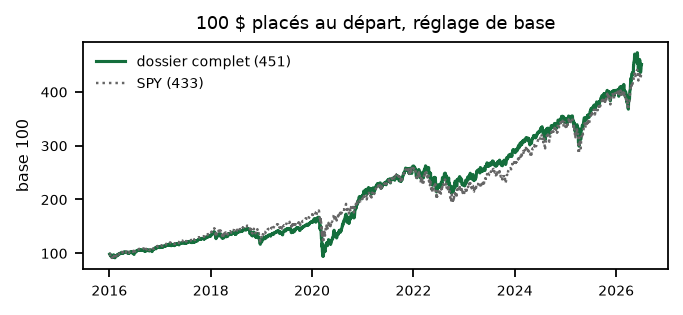
\includegraphics[width=\linewidth]{figures/fig_10_nav.png}\\[1mm]
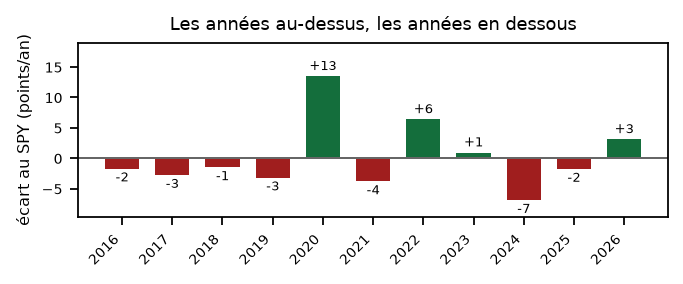
\includegraphics[width=\linewidth]{figures/fig_10_exces_annuel.png}
\end{minipage}

\newpage
% ══════════ PAGE 5 — D'OÙ VIENT LE +6,6 % DE B ? ══════════
\begin{center}
{\Large\bfseries 7 $\cdot$ D'où vient (et ne vient pas) le $+6{,}6\,\%$ de B ?}\\[0.5mm]
{\scriptsize en 10 secondes : le signal vit les années où le top-K est saturé de membres à photo --- et il ne survit pas à la stratification. Sélection, pas information.}
\end{center}

\noindent\begin{minipage}[t]{0.46\textwidth}\vspace{0pt}
\textbf{La matrice des résultats} {\scriptsize(excès/an $\cdot$ $t$, poids $1/K$)}
\begin{center}
\begin{tikzpicture}[x=1cm, y=1cm,
  c/.style 2 args={rectangle, rounded corners=3pt, draw=#1, fill=#1!8, thick,
                   text width=#2, align=center, inner sep=5pt, font=\small}]
\node[c={grisf}{3.4cm}] at (0, 2.6) {\textbf{A} témoin\\ $+0{,}9\,\%$ $\cdot$ $t\,0{,}37$};
\node[c={orange}{3.4cm}] at (4.4, 2.6) {\textbf{C}\\ $-1{,}3\,\%$ $\cdot$ $t\,-0{,}77$};
\node[c={vert}{3.4cm}] at (0, 0) {\textbf{B}\\ $\mathbf{+6{,}6\,\%}$ $\cdot$ $t\,0{,}85$};
\node[c={bleu}{3.4cm}] at (4.4, 0) {\textbf{D} adaptée\\ $-1{,}6\,\%$ $\cdot$ $t\,-0{,}61$};
\end{tikzpicture}
\end{center}
{\scriptsize lecture : la photo seule (B) porte tout l'effet ; les O/A/T (C) pèsent NÉGATIVEMENT ($-2{,}2\,\%$/an apparié) et, combinés (D), effacent B --- les 20\,984 trades tardifs élargissent l'univers (éligibles à la coupe 2021 : de 152 pour A à 241 pour D) et le dégradent.}

\vspace{2mm}
\textbf{S2 --- la même stratégie, par groupe} {\scriptsize(poids $1/K$)}
\begin{center}\small
\begin{tabular}{@{}lrr@{}}
\toprule
strate & excès/an & $t$ \\
\midrule
A $\cdot$ G\_photo & $+0{,}4\,\%$ & $0{,}12$ \\
A $\cdot$ G\_zéro & $-1{,}0\,\%$ & $-0{,}46$ \\
D $\cdot$ G\_photo & $-1{,}1\,\%$ & $-0{,}70$ \\
D $\cdot$ G\_zéro & $-0{,}8\,\%$ & $-0{,}37$ \\
\bottomrule
\end{tabular}
\end{center}
{\scriptsize aucun $t$ stratifié positif : \textbf{le signal ne survit pas à la stratification} --- et la piste \og D$\cdot$G\_zéro \fg{} des versions précédentes s'est évaporée avec les données complétées ($t_{\text{appr}}$ $1{,}59 \to 0{,}59$).}

\vspace{2mm}
\textbf{Puissance} : $\hat\sigma$ des excès annuels $=$ 8,5\,\%/an $\Rightarrow$ \textbf{MDE $\approx$ 6,9\,\%/an}
(excès moyen minimal détectable, $\alpha = 5\,\%$, puissance 80\,\%, $n = 11$). {\scriptsize En dessous, un vrai effet resterait probablement invisible : le nul borne, il ne prouve pas.}
\end{minipage}\hfill
\begin{minipage}[t]{0.51\textwidth}\vspace{0pt}
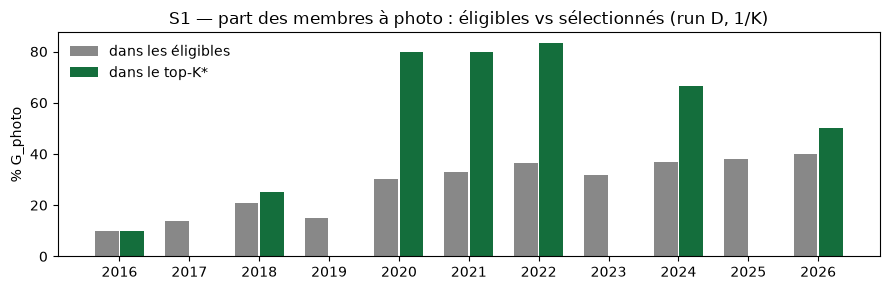
\includegraphics[width=\linewidth]{figures/fig_10_s1.png}\\[1mm]
{\scriptsize \textbf{S1} --- le top-$K$ sur-pondère G\_photo presque toutes les années (jusqu'à 67\,\% du panier contre $\sim$30\,\% des éligibles ; seul 2019 est à 0\,\%). $K^*$ walk-forward : B verrouille $K{=}4$ ; C et D montent en $K$ (8-18, puis $\sim$11) --- l'univers élargi disperse ; la sélection A vs D diffère à 11/11 coupes.}
\end{minipage}

\newpage
% ══════════ PAGE 6 — QUE CONCLURE ? ══════════
\begin{center}
{\Large\bfseries 8 $\cdot$ Que conclure --- et pourquoi y croire ?}
\end{center}

\noindent\begin{minipage}[t]{0.47\textwidth}\vspace{0pt}
\textbf{\color{rouge}Verdict}
\begin{itemize}
\item[--] \textbf{pas d'alpha démontrable} : $\max t = 0{,}85$, effets appariés nuls, $t$ appariés stratifiés $\le 0{,}59$ --- robuste au poids, à la strate, et au périmètre (et il se renforce quand on complète les données : D $-1{,}6\,\%$/an) ;
\item[--] les corrections rendent la mesure \textbf{plus honnête}, pas plus rentable : $\beta$ $0{,}99 \to 0{,}85$, effet O/A/T négatif --- mais la \textbf{reconstruction} est $10\times$ plus complète (rappel 6\,\% $\to$ 57\,\%, p.\,5) ;
\item[--] le seul effet positif (photo, $+6{,}6\,\%$) coïncide avec les années où le top-$K$ est saturé de G\_photo --- \textbf{mesure plutôt que talent}.
\end{itemize}

\vspace{1mm}
\textbf{A $\to$ D, ce qui s'améliore}
\begin{center}\small
\begin{tabular}{@{}lccc@{}}
\toprule
 & A témoin & D adaptée & \\
\midrule
membres couverts & 226 & \textbf{400} & $\nearrow$ \\
photos injectées & 0 & \textbf{160} & $\nearrow$ \\
$\beta$ & 0,99 & \textbf{0,85} & $\searrow$ \\
$t_{\alpha}$ ajusté & $+0{,}28$ & $+0{,}37$ & $\approx$ \\
excès/an & $+0{,}9\,\%$ & $-1{,}6\,\%$ & $\searrow$ \\
\bottomrule
\end{tabular}
\end{center}

\vspace{1mm}
\textbf{\color{grisf}Pourquoi y croire} {\scriptsize : recalcul naïf 869 rendements identiques $\cdot$ $r = 0$ au jour d'injection $\cdot$ B $\equiv$ A hors photos $\cdot$ bloc 2018 refait à la main $\cdot$ \texttt{prices\_v2} intact $\cdot$ cascades vérifiées par assert.}
\end{minipage}\hfill
\begin{minipage}[t]{0.50\textwidth}\vspace{0pt}
\textbf{Limites --- et le test qui trancherait chacune}
\begin{center}\small
\begin{tabularx}{\linewidth}{@{}XXX@{}}
\toprule
limite & conséquence & test qui trancherait \\
\midrule
O/A/T datés à la transaction, divulgués $\sim$374 j après & C et D optimistes par construction (pas jouables tels quels) & re-dater les O/A/T au jour du dépôt --- devrait tuer C \\
double comptage possible (achat PTR pré-dépôt $\subset$ photo) & $h_0$ surestimé pour certains & re-jouer B sans les PTR antérieurs au dépôt \\
24,7\,\% de la valeur des photos non convertie (non-coté) & G\_photo partiellement observé & --- (limite de données) \\
coûts de transaction non modélisés & tout excès net serait plus bas & grille de coûts (5-20 bps) \\
$n = 11$ années & puissance limitée (MDE 6,9\,\%/an) & attendre, ou passer en coupes semestrielles \\
\bottomrule
\end{tabularx}
\end{center}

\vspace{1mm}
\textbf{La valeur du travail, même sous le null} : le pipeline de données est réparé --- 437 traders au lieu de 305, une reconstruction vérifiée contre 2\,173 photos annuelles (rappel 6\,\% $\to$ 57\,\%) --- et sert tel quel à toute stratégie future (ticker, notebook 11).
\end{minipage}

\end{document}
